In Model 3, the cell was treated as a point particle, neglecting the effects of cell shape on boundary interactions. 
To address this limitation, we explored incorporating cell geometry explicitly into Model 3, aiming to understand how the 
resulting PDF would compare to the shape0-dependent outcomes observed in Models 1 and 2.

This integration of shape could be implemented through multiple approaches. Our chosen method involved redistribution 
the probability mass from the boundary accumulation peaks observed in the marginal distirbution along $y$ (see Figure 
\ref{fig:model_3_hist}) over a finite region corresponding to the physical contact of an elliptical cell with the 
channel walls. Specifically, we computed the geometric average distance of an elliptically shaped cell from the 
wall and redistributed the probability previously representing 
point-particle capture in Model 3, were distirbuted. The computed average boundary distance for an ellipse is
illustrated by the solid red line in Figure \ref{fig:average_boundary}.

\begin{figure}[htbp]
    \centering
    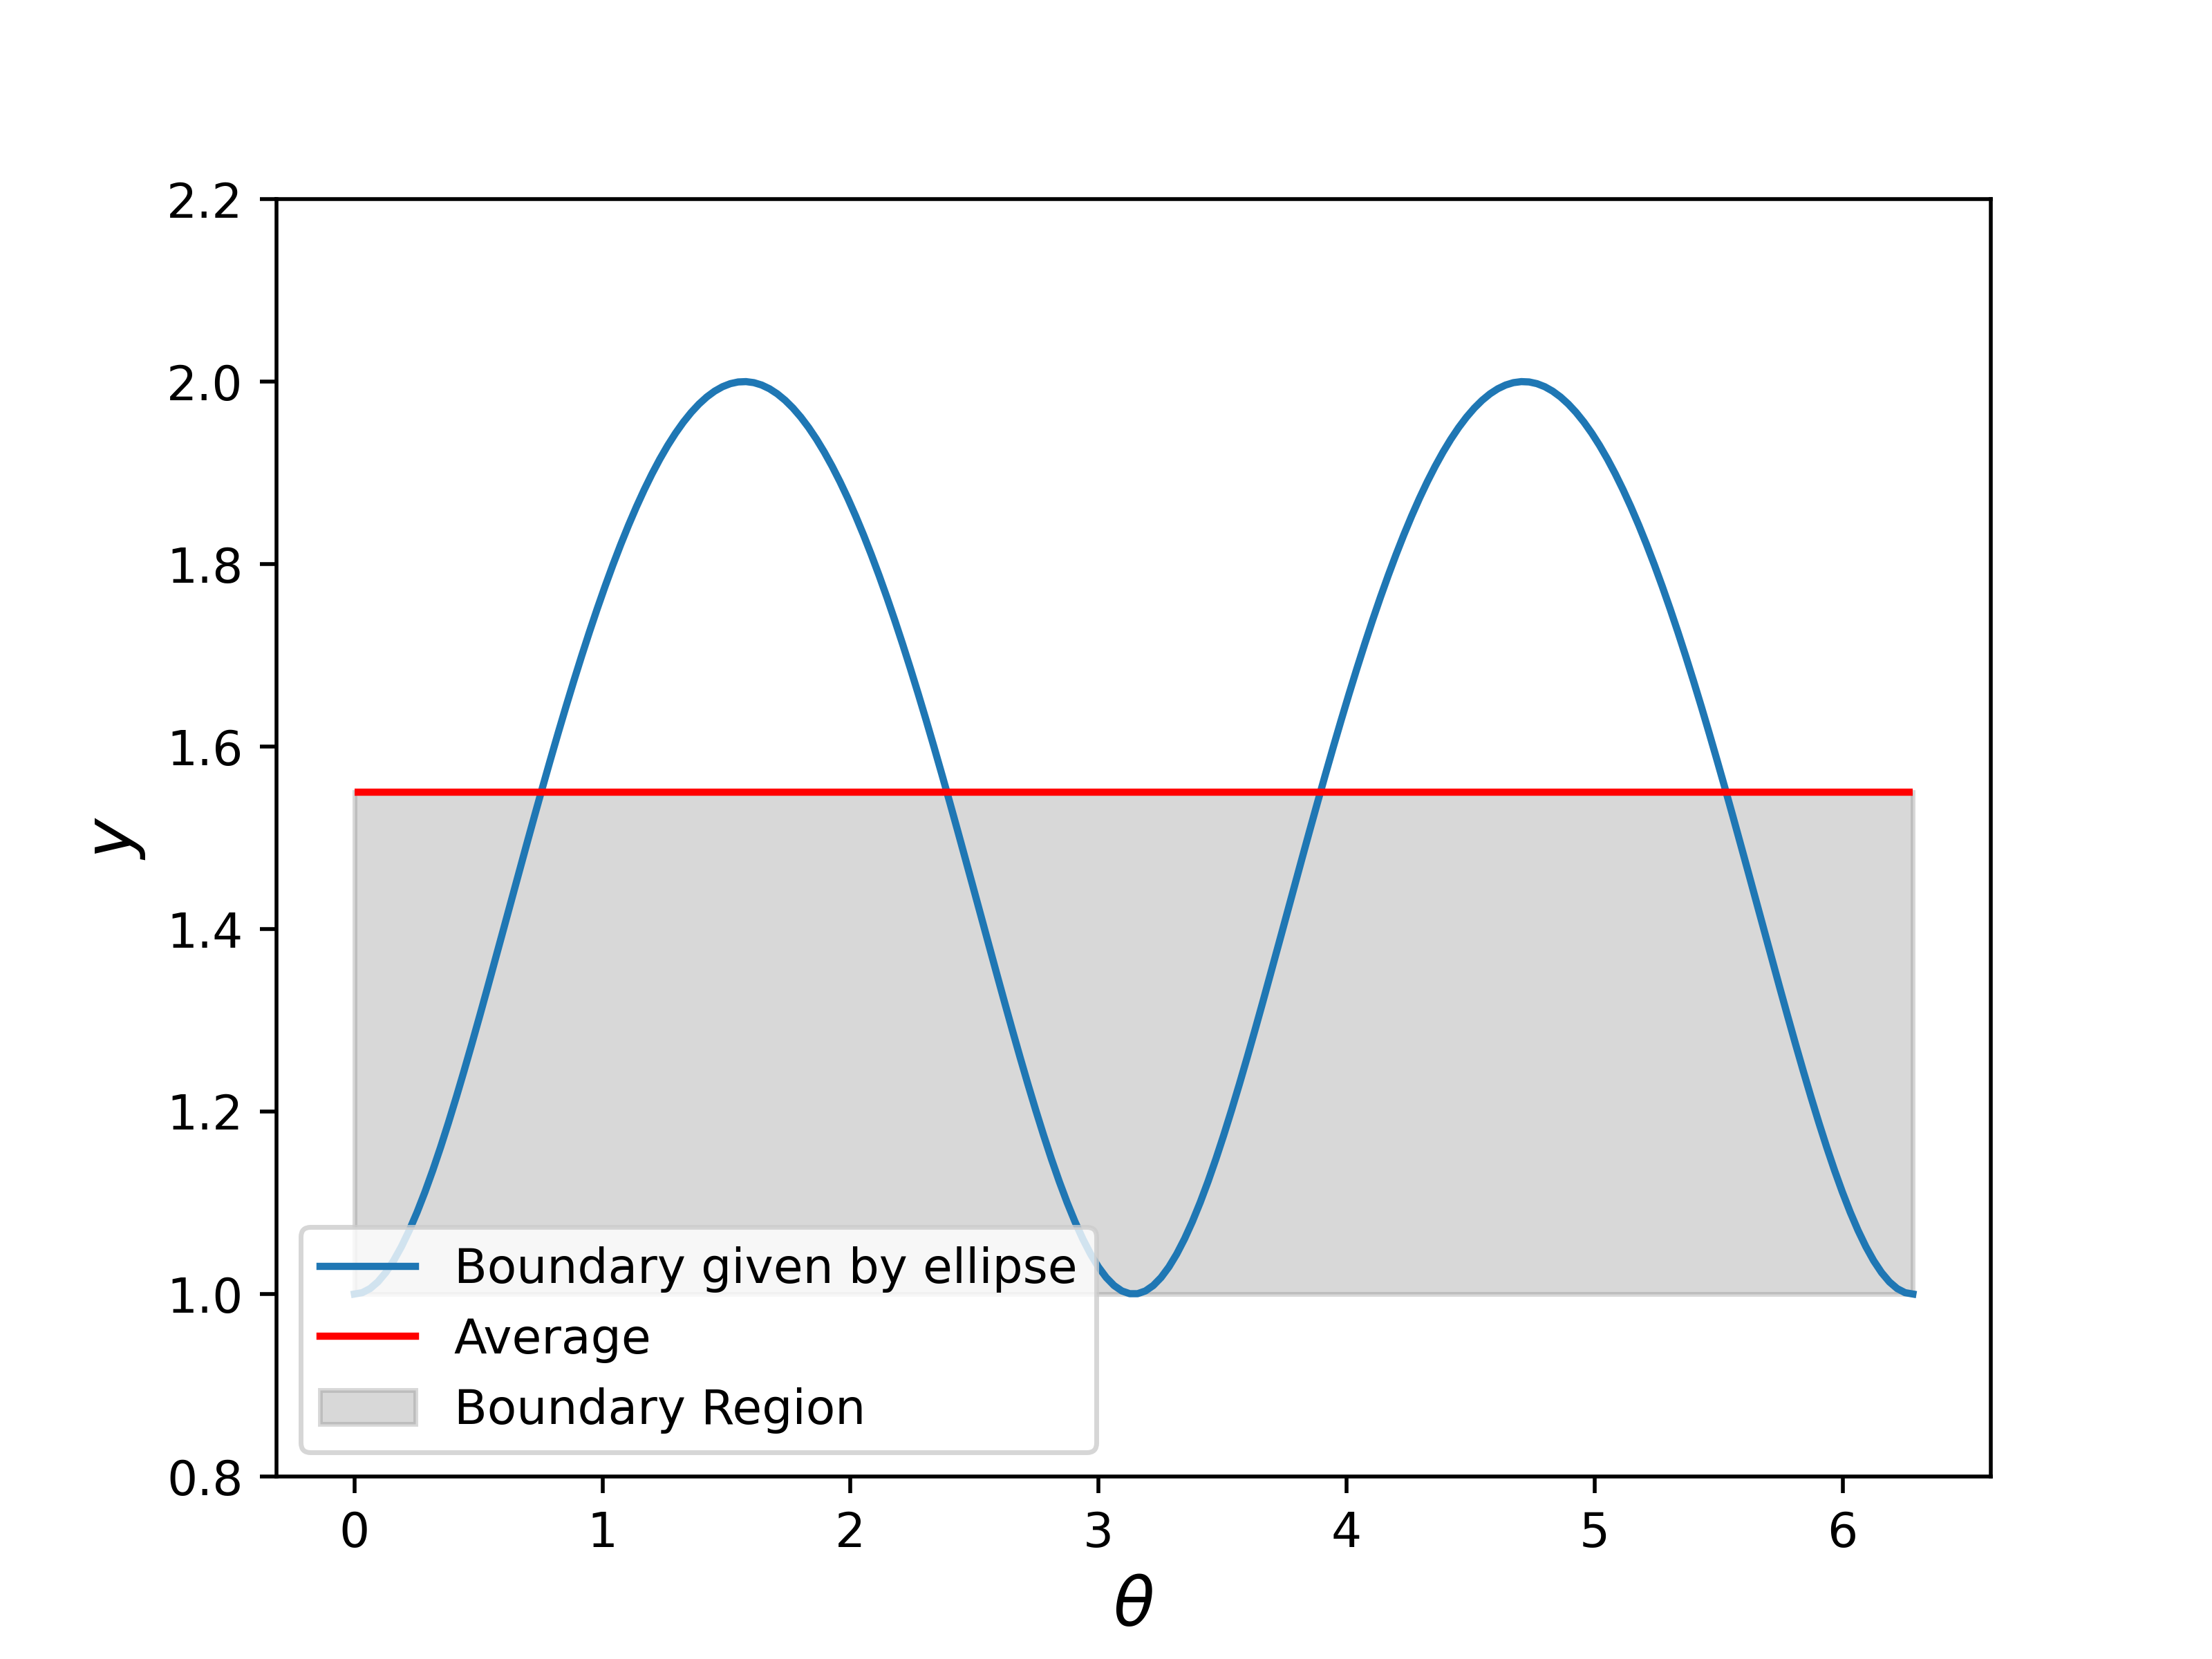
\includegraphics[scale=0.4]{graphics/average_boundary.png}
    \caption{Illustration of methodology for redistributing boundary-accumulated 
    probability mass based on the geometric average boundary distance of an elliptical cell.}
    \label{fig:average_boundary}
\end{figure}

The average was calculated as $\bar{y} = \frac{1}{2\pi}\int_{0}^{2\pi}\sqrt{a^2\sin^2(\theta) + b^2\cos^2(\theta)}$,
where the integrand corresponds to the wall distance function previously defined in \eqref{eq:wall_dist_funcs}.
The resulting adjusted marginal distribution is given in Figure \ref{fig:model_3_modified_hist}.

\begin{figure}[htbp]
    \centering
    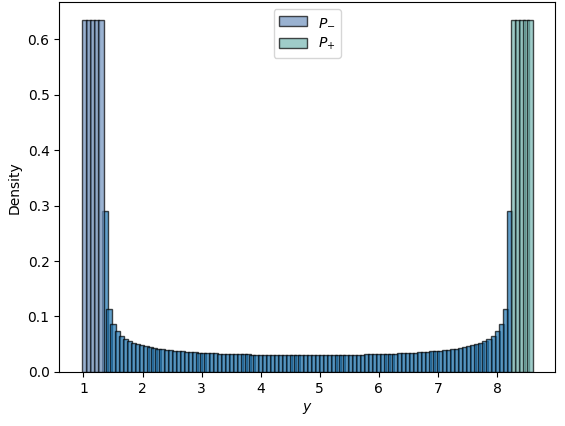
\includegraphics[scale=0.4]{graphics/model_3_with_shape_hist.png}
    \caption{Marginal distribution after redistributing Model 3's boundary-accumulated probability mass according to the cell
    shape.}
    \label{fig:model_3_modified_hist}. 
\end{figure}

Finally, we compared the marginal distributions from Model 1, Model 2 and the modified version of Model 3.
These distributions, generated with identical parameters for consistency, are shown in 
Figure \ref{fig:model_comparisons}.

\begin{figure}[htbp]
    \centering
    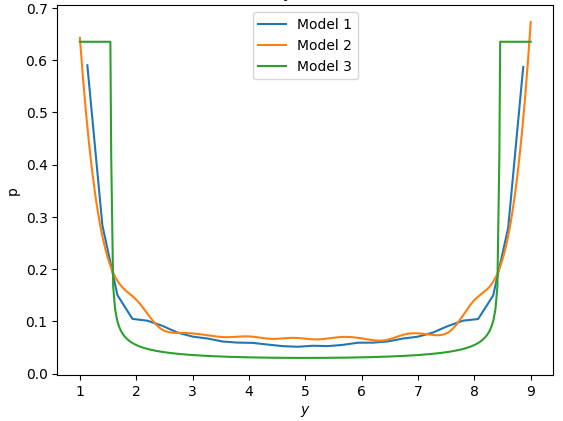
\includegraphics[scale=0.4]{graphics/model_comparisons.png}
    \caption{Comparison of Marginal PDFs from Model 1, Model 2, and the shape-adjusted Model 3.}
    \label{fig:model_comparisons}. 
\end{figure}

From Figure \ref{fig:model_comparisons}, Models 1 and 2 show close alignment, suggesting that additional hydrodynamic
terms in Model 2 may have a relatively minor effect on boundary accumulation under the conditions investigated here.
Further investigation through additional simulations and parameter variations is recommended to comprehensively 
understand the conditions under which hydrodynamic interactions significantly influence the observed cell behavior.

In contrast, Model 3 assigns more probability mass at the boundaries compared to Models 1 and 2. This discrepancy 
suggests that the simplistic bonudary interactions in Model 3 may overestimate the boundary accumulatino effect.

For future work, several extensions can be considered:

\begin{itemize}
    \item Investigate imposing Robin boundary conditions to more accurately capture 
    interactions between cells and boundaries.
    \item Adjusting the cell's centre of rotation, which may usbstantially influence boundary accumulation
    phenomena, as is expored in \cite{chen2021shape}.
    \item Investigating the effects of alternative cell shapes beyond ellipses to generalise the results
    \item Exploring boundary accumulation behaviour near complex boundaries or obstacles, such as circular or 
    irregular shapes within the channel.
    \item Considering collective interactions among the multiple cells to understand how inter-cellular dynamics affect 
    boundary accumulation. 
\end{itemize}


